\documentclass{standalone}
\usepackage{tikz}
\usetikzlibrary{patterns, positioning}
\usepackage[sfdefault]{ClearSans} %% option 'sfdefault' activates Clear Sans as the default text font
\usepackage[T1]{fontenc}

\begin{document}
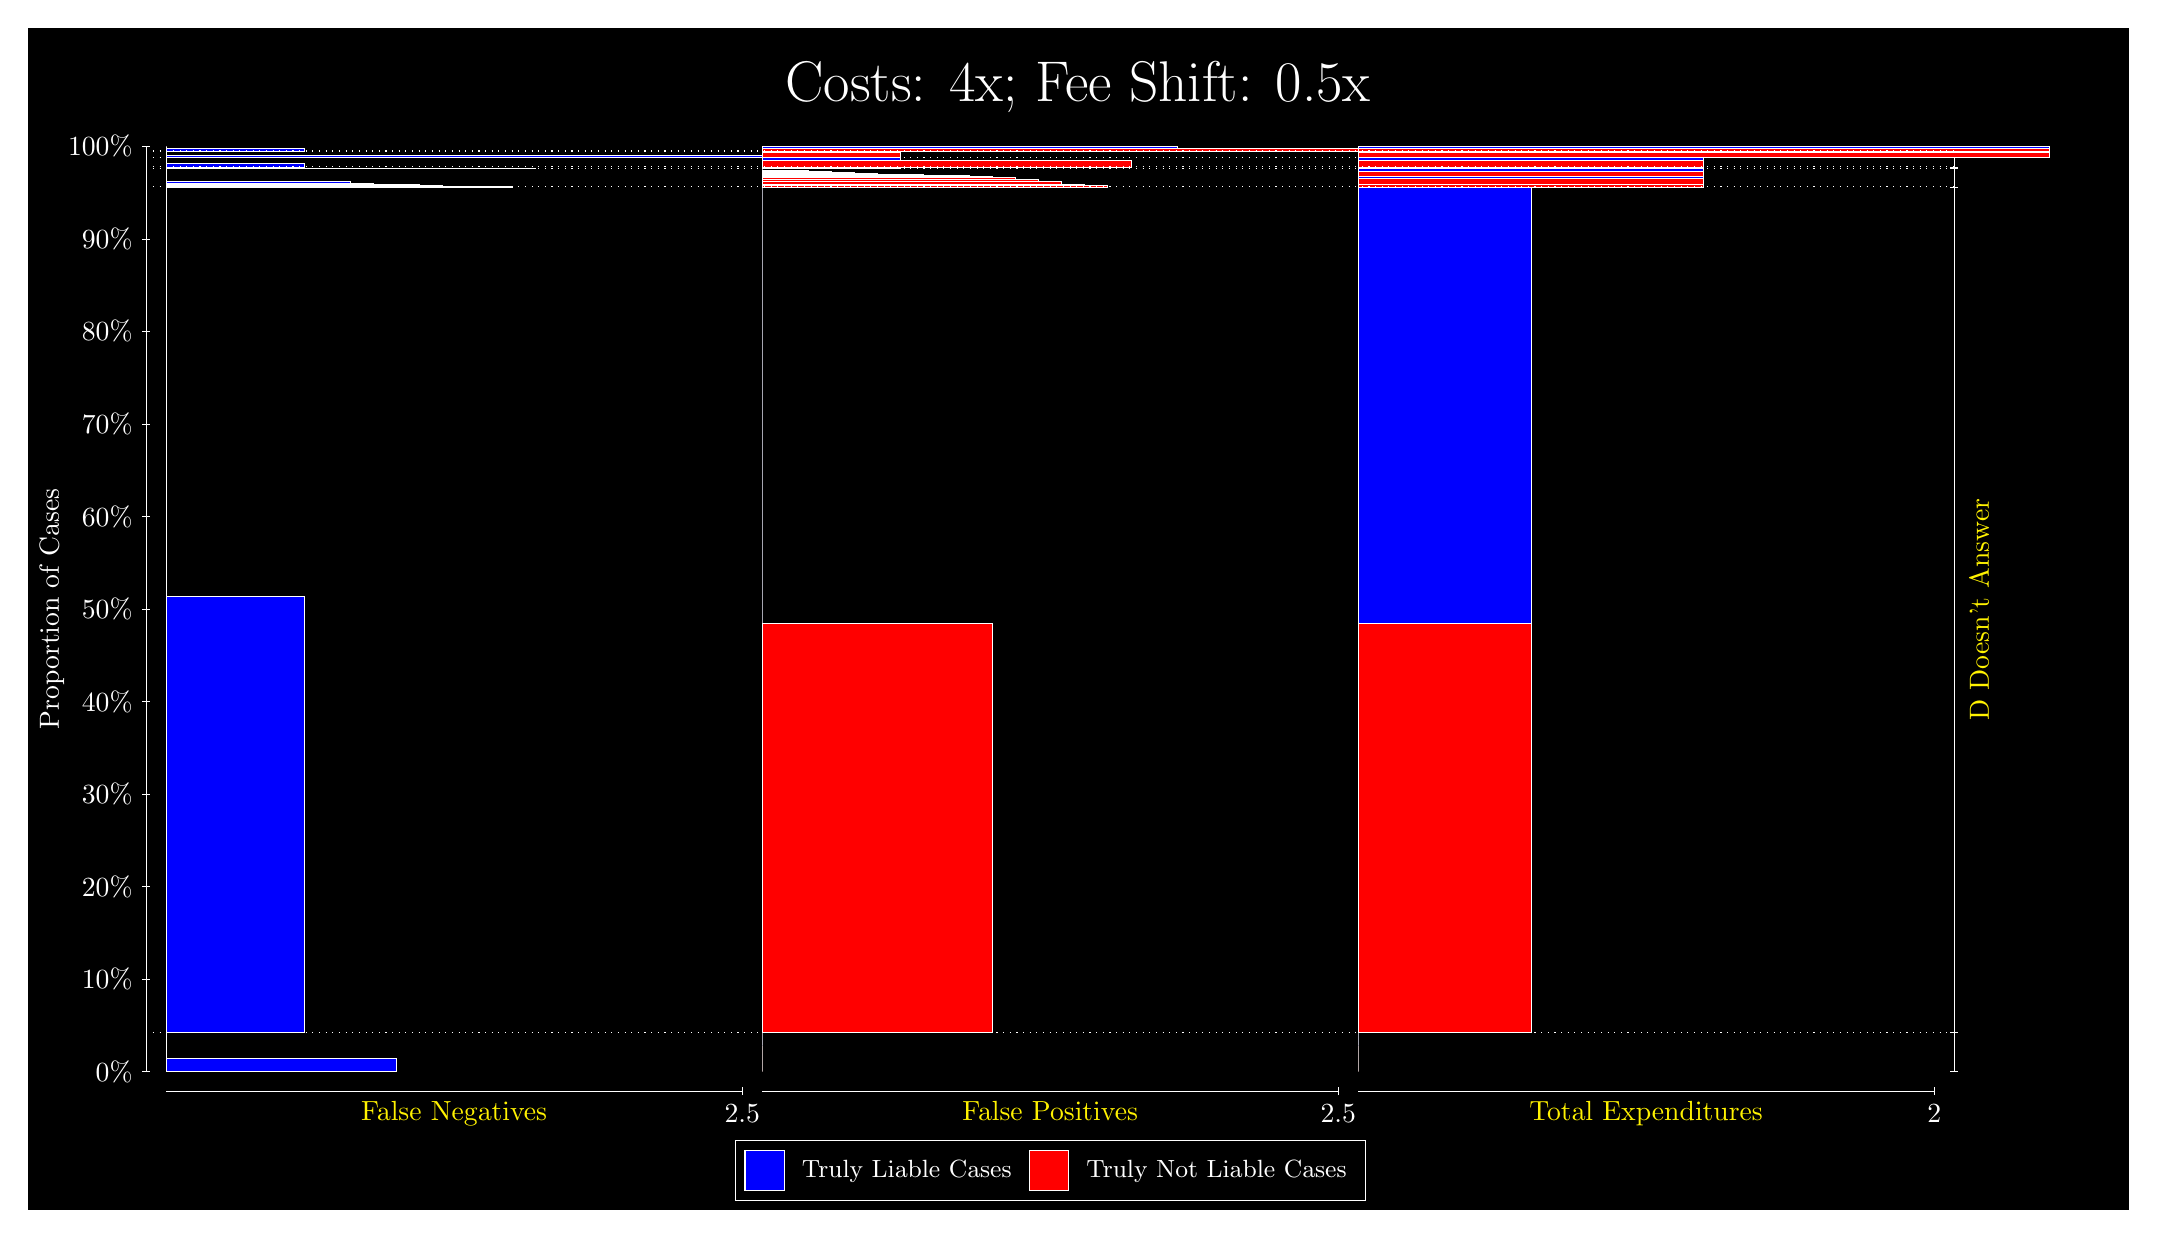
\begin{tikzpicture}
\draw[fill=black] (0,0) rectangle (26.667,15);
\draw[text=white] (0,13.5) rectangle (26.667,15) node[midway] {\huge Costs: 4x; Fee Shift: 0.5x};
\draw[white, very thin] (1.5,1.75) -- (1.5,13.5);
\node[rotate=90, text=white, anchor=center] at (0.3, 7.625) {Proportion of Cases};
\draw[white, very thin] (1.45,1.75) -- (1.55,1.75);
\node[text=white, anchor=east] at (1.45, 1.75) {0\%};
\draw[white, very thin] (1.45,2.925) -- (1.55,2.925);
\node[text=white, anchor=east] at (1.45, 2.925) {10\%};
\draw[white, very thin] (1.45,4.1) -- (1.55,4.1);
\node[text=white, anchor=east] at (1.45, 4.1) {20\%};
\draw[white, very thin] (1.45,5.275) -- (1.55,5.275);
\node[text=white, anchor=east] at (1.45, 5.275) {30\%};
\draw[white, very thin] (1.45,6.45) -- (1.55,6.45);
\node[text=white, anchor=east] at (1.45, 6.45) {40\%};
\draw[white, very thin] (1.45,7.625) -- (1.55,7.625);
\node[text=white, anchor=east] at (1.45, 7.625) {50\%};
\draw[white, very thin] (1.45,8.8) -- (1.55,8.8);
\node[text=white, anchor=east] at (1.45, 8.8) {60\%};
\draw[white, very thin] (1.45,9.975) -- (1.55,9.975);
\node[text=white, anchor=east] at (1.45, 9.975) {70\%};
\draw[white, very thin] (1.45,11.15) -- (1.55,11.15);
\node[text=white, anchor=east] at (1.45, 11.15) {80\%};
\draw[white, very thin] (1.45,12.325) -- (1.55,12.325);
\node[text=white, anchor=east] at (1.45, 12.325) {90\%};
\draw[white, very thin] (1.45,13.5) -- (1.55,13.5);
\node[text=white, anchor=east] at (1.45, 13.5) {100\%};

\draw[white, very thin] (24.457,1.75) -- (24.457,13.5);
\draw[white, very thin] (24.407,1.75) -- (24.507,1.75);
\node[anchor=west] at (24.407, 1.75) {};
\draw[white, very thin] (24.407,2.2431) -- (24.507,2.2431);
\node[anchor=west] at (24.407, 2.2431) {};
\draw[white, very thin] (24.407,12.986) -- (24.507,12.986);
\node[anchor=west] at (24.407, 12.986) {};
\draw[white, very thin] (24.407,13.215) -- (24.507,13.215);
\node[anchor=west] at (24.407, 13.215) {};
\draw[white, very thin] (24.407,13.24) -- (24.507,13.24);
\node[anchor=west] at (24.407, 13.24) {};
\draw[white, very thin] (24.407,13.363) -- (24.507,13.363);
\node[anchor=west] at (24.407, 13.363) {};
\draw[white, very thin] (24.407,13.441) -- (24.507,13.441);
\node[anchor=west] at (24.407, 13.441) {};
\draw[white, very thin] (24.407,13.5) -- (24.507,13.5);
\node[anchor=west] at (24.407, 13.5) {};

\draw[white, very thin, fill=blue] (1.75,1.75) rectangle (4.6775,1.9134);
\draw[white, very thin, fill=red] (1.75,1.9134) rectangle (1.75,2.2431);
\draw[white, very thin, fill=blue] (1.75,2.2431) rectangle (3.5065,7.7816);
\draw[white, very thin, fill=red] (1.75,7.7816) rectangle (1.75,12.986);
\draw[white, very thin, fill=blue] (1.75,12.986) rectangle (6.1413,12.991);
\draw[white, very thin, fill=blue] (1.75,12.991) rectangle (5.8486,12.993);
\draw[white, very thin, fill=blue] (1.75,12.993) rectangle (5.5558,12.998);
\draw[white, very thin, fill=blue] (1.75,12.998) rectangle (5.2631,13.002);
\draw[white, very thin, fill=blue] (1.75,13.002) rectangle (4.9703,13.012);
\draw[white, very thin, fill=blue] (1.75,13.012) rectangle (4.6775,13.018);
\draw[white, very thin, fill=blue] (1.75,13.018) rectangle (4.3848,13.037);
\draw[white, very thin, fill=blue] (1.75,13.037) rectangle (4.092,13.05);
\draw[white, very thin, fill=blue] (1.75,13.05) rectangle (3.7993,13.058);
\draw[white, very thin, fill=red] (1.75,13.058) rectangle (1.75,13.215);
\draw[white, very thin, fill=blue] (1.75,13.215) rectangle (6.4341,13.221);
\draw[white, very thin, fill=red] (1.75,13.221) rectangle (1.75,13.24);
\draw[white, very thin, fill=blue] (1.75,13.24) rectangle (3.5065,13.285);
\draw[white, very thin, fill=red] (1.75,13.285) rectangle (1.75,13.363);
\draw[white, very thin, fill=blue] (1.75,13.363) rectangle (9.9471,13.384);
\draw[white, very thin, fill=red] (1.75,13.384) rectangle (1.75,13.441);
\draw[white, very thin, fill=blue] (1.75,13.441) rectangle (3.5065,13.471);
\draw[white, very thin, fill=red] (1.75,13.471) rectangle (1.75,13.5);
\draw[white, very thin, fill=red] (9.3189,1.75) rectangle (9.3189,2.0798);
\draw[white, very thin, fill=blue] (9.3189,2.0798) rectangle (9.3189,2.2431);
\draw[white, very thin, fill=red] (9.3189,2.2431) rectangle (12.246,7.4481);
\draw[white, very thin, fill=blue] (9.3189,7.4481) rectangle (9.3189,12.986);
\draw[white, very thin, fill=red] (9.3189,12.986) rectangle (13.71,13);
\draw[white, very thin, fill=red] (9.3189,13) rectangle (13.417,13.023);
\draw[white, very thin, fill=red] (9.3189,13.023) rectangle (13.125,13.06);
\draw[white, very thin, fill=red] (9.3189,13.06) rectangle (12.832,13.08);
\draw[white, very thin, fill=red] (9.3189,13.08) rectangle (12.539,13.106);
\draw[white, very thin, fill=red] (9.3189,13.106) rectangle (12.246,13.117);
\draw[white, very thin, fill=red] (9.3189,13.117) rectangle (11.954,13.128);
\draw[white, very thin, fill=red] (9.3189,13.128) rectangle (11.661,13.134);
\draw[white, very thin, fill=red] (9.3189,13.134) rectangle (11.368,13.143);
\draw[white, very thin, fill=blue] (9.3189,13.143) rectangle (10.783,13.152);
\draw[white, very thin, fill=blue] (9.3189,13.152) rectangle (10.49,13.165);
\draw[white, very thin, fill=blue] (9.3189,13.165) rectangle (10.197,13.183);
\draw[white, very thin, fill=blue] (9.3189,13.183) rectangle (9.9044,13.19);
\draw[white, very thin, fill=blue] (9.3189,13.19) rectangle (9.6116,13.199);
\draw[white, very thin, fill=blue] (9.3189,13.199) rectangle (9.3189,13.215);
\draw[white, very thin, fill=red] (9.3189,13.215) rectangle (11.075,13.234);
\draw[white, very thin, fill=blue] (9.3189,13.234) rectangle (9.3189,13.24);
\draw[white, very thin, fill=red] (9.3189,13.24) rectangle (14.003,13.318);
\draw[white, very thin, fill=blue] (9.3189,13.318) rectangle (11.075,13.363);
\draw[white, very thin, fill=red] (9.3189,13.363) rectangle (11.075,13.42);
\draw[white, very thin, fill=blue] (9.3189,13.42) rectangle (9.3189,13.441);
\draw[white, very thin, fill=red] (9.3189,13.441) rectangle (17.516,13.47);
\draw[white, very thin, fill=blue] (9.3189,13.47) rectangle (14.588,13.5);
\draw[white, very thin, fill=red] (16.888,1.75) rectangle (16.888,2.0798);
\draw[white, very thin, fill=blue] (16.888,2.0798) rectangle (16.888,2.2431);
\draw[white, very thin, fill=red] (16.888,2.2431) rectangle (19.083,7.4481);
\draw[white, very thin, fill=blue] (16.888,7.4481) rectangle (19.083,12.986);
\draw[white, very thin, fill=red] (16.888,12.986) rectangle (21.279,13.012);
\draw[white, very thin, fill=blue] (16.888,13.012) rectangle (21.279,13.022);
\draw[white, very thin, fill=red] (16.888,13.022) rectangle (21.279,13.092);
\draw[white, very thin, fill=blue] (16.888,13.092) rectangle (21.279,13.123);
\draw[white, very thin, fill=red] (16.888,13.123) rectangle (21.279,13.183);
\draw[white, very thin, fill=blue] (16.888,13.183) rectangle (21.279,13.215);
\draw[white, very thin, fill=red] (16.888,13.215) rectangle (21.279,13.234);
\draw[white, very thin, fill=blue] (16.888,13.234) rectangle (21.279,13.24);
\draw[white, very thin, fill=red] (16.888,13.24) rectangle (21.279,13.318);
\draw[white, very thin, fill=blue] (16.888,13.318) rectangle (21.279,13.363);
\draw[white, very thin, fill=red] (16.888,13.363) rectangle (25.67,13.42);
\draw[white, very thin, fill=blue] (16.888,13.42) rectangle (25.67,13.441);
\draw[white, very thin, fill=red] (16.888,13.441) rectangle (25.67,13.47);
\draw[white, very thin, fill=blue] (16.888,13.47) rectangle (25.67,13.5);
\draw[white, dotted] (1.5,2.2431) -- (24.457,2.2431);
\draw[white, dotted] (1.5,12.986) -- (24.457,12.986);
\draw[white, dotted] (1.5,13.215) -- (24.457,13.215);
\draw[white, dotted] (1.5,13.24) -- (24.457,13.24);
\draw[white, dotted] (1.5,13.363) -- (24.457,13.363);
\draw[white, dotted] (1.5,13.441) -- (24.457,13.441);
\draw[white, very thin] (1.75,1.5) -- (9.0689,1.5);
\node[text=yellow, anchor=north] at (5.4094, 1.5) {False Negatives};
\draw[white, very thin] (9.0689,1.45) -- (9.0689,1.55);
\node[text=white, anchor=north] at (9.0689, 1.45) {2.5};

\draw[white, very thin] (9.3189,1.5) -- (16.638,1.5);
\node[text=yellow, anchor=north] at (12.978, 1.5) {False Positives};
\draw[white, very thin] (16.638,1.45) -- (16.638,1.55);
\node[text=white, anchor=north] at (16.638, 1.45) {2.5};

\draw[white, very thin] (16.888,1.5) -- (24.207,1.5);
\node[text=yellow, anchor=north] at (20.547, 1.5) {Total Expenditures};
\draw[white, very thin] (24.207,1.45) -- (24.207,1.55);
\node[text=white, anchor=north] at (24.207, 1.45) {2};


\node[text=yellow, centered, rotate=90] at (24.777, 7.6148) {D Doesn't Answer};






\draw (12.978300999999998,1.5) node[draw=none] (baseCoordinate) {};
\begin{scope}[align=center]
        \matrix[scale=0.5, draw=white, below=0.5cm of baseCoordinate, nodes={draw}, column sep=0.1cm]{
            \node[rectangle, draw, minimum width=0.5cm, minimum height=0.5cm, fill=blue] {}; &
            \node[draw=none, font=\small, text=white] (B) {Truly Liable Cases}; &
            \node[rectangle, draw, minimum width=0.5cm, minimum height=0.5cm, fill=red] {}; &
            \node[draw=none, font=\small, text=white] (B) {Truly Not Liable Cases}; \\
            };
\end{scope}

\end{tikzpicture}
\end{document}